\section{Belief propagation}

Belief propagation, often referred to as message passing, bears similarities to the variable elimination algorithm.
This approach is amenable to parallel execution at each node, where it computes messages exchanged between variables and factors.
It can be summarized in two fundamental steps: message computation and probability estimation based on the derived messages.
In cases of circular dependencies, this method is effective when applied to a graph structured as a tree or polytree (a tree with no designated root).

It's important to note that messages in belief propagation correspond to the $\mu$ factors in the variable elimination algorithm, with leaf $\mu$ factors always initialized to 1.
To initiate the algorithm, we require message values from a prior state, making it practical to start from the leaf nodes.

As previously mentioned, belief propagation can be expressed as a parallel procedure that adheres to the following steps:
\begin{enumerate}
    \item Initialization of all messages:
        \[\mu_{f_s\rightarrow X_i}= 1\]
        \[\mu_{X_i \rightarrow f_s}= 1\]
    \item Message updates:
        \[\mu_{f_s\rightarrow X_i}^{new}(X_i)=\sum_{X_s \backslash X_i}f_s(X_i,X_s)\prod_{X_j \in new(X_i), j \neq i}\mu_{X_i \rightarrow f_s}^{old}(X_j)\]
        \[\mu_{X_i \rightarrow f_s}^{new}(X_i)=\prod_{f_l \in new(X_i),f_l \neq f_s}\mu_{f_l \rightarrow X_i}^{old}(X_i)\]
    \item Belief updates:
        \[b_{f_s}(X_s)=f_s(X_s) \prod_{j \in f_s}\mu_{X_j \rightarrow f_s}(X_j)\]
        \[b_{X_i}(X_i)=\prod_{f_s \in new(i)}\mu_{f_s \rightarrow X_i}(X_i)\]
\end{enumerate}
This iterative procedure is executed until convergence is achieved.
\begin{example}
    Consider the Bayesian network shown below along with the associated probabilities:
    \begin{figure}[H]
        \centering
        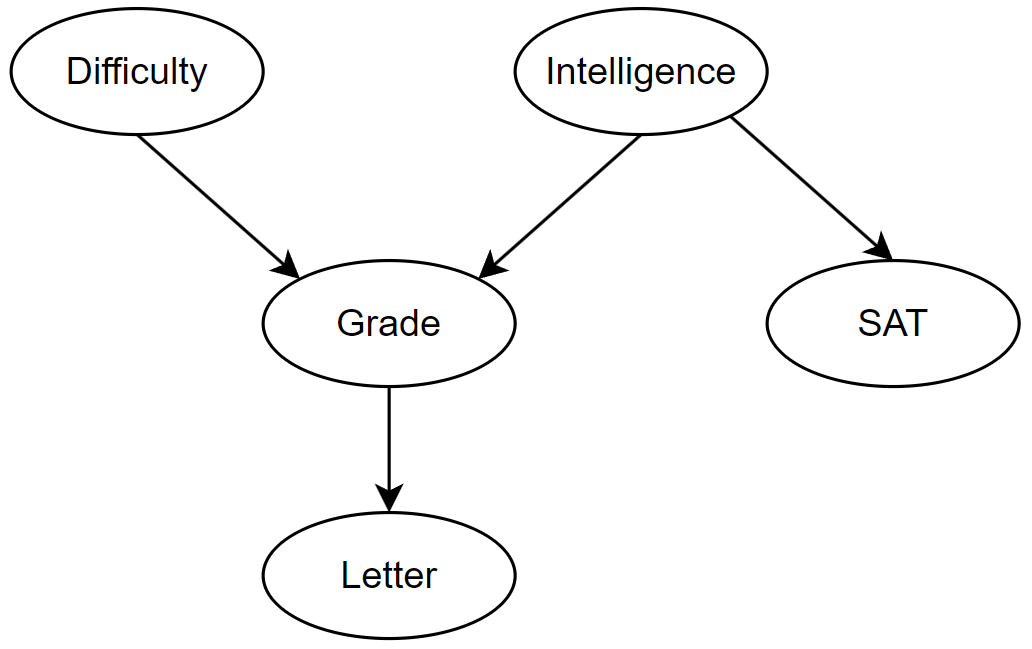
\includegraphics[width=0.5\linewidth]{images/bay.png}
    \end{figure}
    With these probabilities: 
    \begin{table}[H]
        \centering
        \begin{tabular}{|cc|}
        \hline
        $d^0$ & $d^1$ \\ \hline
        0.6   & 0.4   \\ \hline
        \end{tabular}
    \end{table}
    \begin{table}[H]
        \centering
        \begin{tabular}{|cc|}
        \hline
        $i^0$ & $i^1$ \\ \hline
        0.7   & 0.3   \\ \hline
        \end{tabular}
    \end{table}
    \begin{table}[H]
        \centering
        \begin{tabular}{c|cc|}
        \cline{2-3}
                                    & $s^0$ & $s^1$ \\ \hline
        \multicolumn{1}{|c|}{$i^0$} & 0.95  & 0.05  \\
        \multicolumn{1}{|c|}{$i^1$} & 0.2   & 0.8   \\ \hline
        \end{tabular}
    \end{table}
    \begin{table}[H]
        \centering
        \begin{tabular}{c|cc|}
        \cline{2-3}
                                    & $l^0$ & $l^1$ \\ \hline
        \multicolumn{1}{|c|}{$g^1$} & 0.1   & 0.9   \\
        \multicolumn{1}{|c|}{$g^2$} & 0.4   & 0.6   \\
        \multicolumn{1}{|c|}{$g^3$} & 0.99  & 0.01  \\ \hline
        \end{tabular}
    \end{table}
    \begin{table}[H]
        \centering
        \begin{tabular}{c|ccc|}
        \cline{2-4}
                                        & $g^1$ & $g^2$ & $g^3$ \\ \hline
        \multicolumn{1}{|c|}{$i^0,d^0$} & 0.3   & 0.4   & 0.3   \\
        \multicolumn{1}{|c|}{$i^0,d^1$} & 0.05  & 0.25  & 0.7   \\
        \multicolumn{1}{|c|}{$i^1,d^0$} & 0.9   & 0.08  & 0.02  \\
        \multicolumn{1}{|c|}{$i^1,d^1$} & 0.5   & 0.3   & 0.2   \\ \hline
        \end{tabular}
    \end{table}
    From this network, we create the corresponding factor graph:
    \begin{figure}[H]
        \centering
        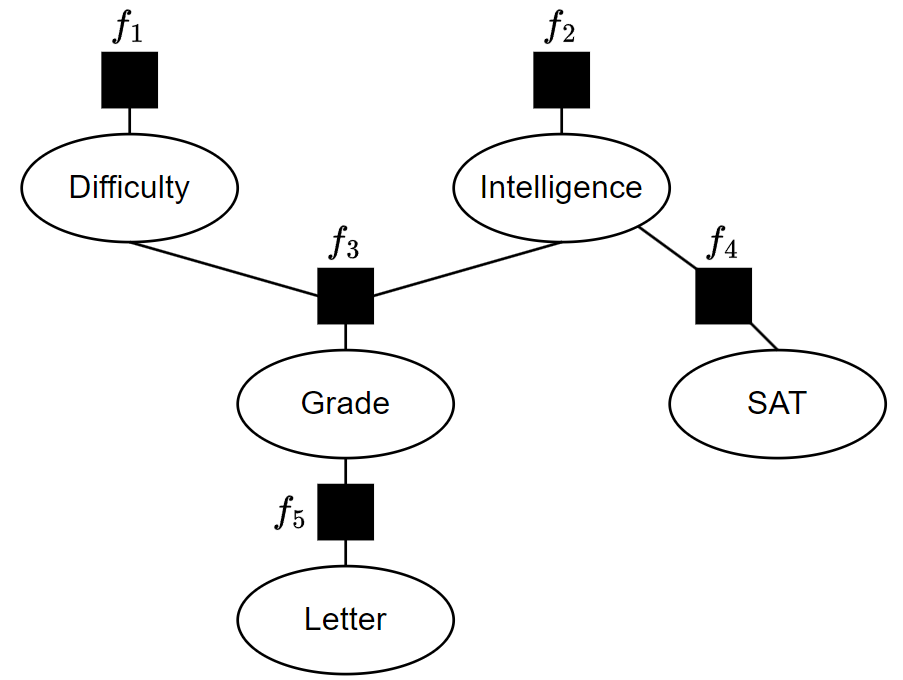
\includegraphics[width=0.5\linewidth]{images/bayfac.png}
    \end{figure}
    The corresponding functions are: 
    \begin{table}[H]
        \centering
        \begin{tabular}{c|c|}
        \cline{2-2}
        $D$                     & $f_1(D)$ \\ \hline
        \multicolumn{1}{|c|}{0} & 0.6      \\
        \multicolumn{1}{|c|}{1} & 0.4      \\ \hline
        \end{tabular}
    \end{table}
    \begin{table}[H]
        \centering
        \begin{tabular}{c|c|}
        \cline{2-2}
        $I$                     & $f_2(I)$ \\ \hline
        \multicolumn{1}{|c|}{0} & 0.7      \\
        \multicolumn{1}{|c|}{1} & 0.3      \\ \hline
        \end{tabular}
    \end{table}
    \begin{table}[H]
        \centering
        \begin{tabular}{ccc|c|}
        \cline{4-4}
        $G$                    & $I$ & $D$ & $f_3(G,I,D)$ \\ \hline
        \multicolumn{1}{|c}{1} & 0   & 0   & 0.3          \\
        \multicolumn{1}{|c}{1} & 0   & 1   & 0.05         \\
        \multicolumn{1}{|c}{1} & 1   & 0   & 0.9          \\
        \multicolumn{1}{|c}{1} & 1   & 1   & 0.5          \\
        \multicolumn{1}{|c}{2} & 0   & 0   & 0.4          \\
        \multicolumn{1}{|c}{2} & 0   & 1   & 0.25         \\
        \multicolumn{1}{|c}{2} & 1   & 0   & 0.08         \\
        \multicolumn{1}{|c}{2} & 1   & 1   & 0.3          \\
        \multicolumn{1}{|c}{3} & 0   & 0   & 0.3          \\
        \multicolumn{1}{|c}{3} & 0   & 1   & 0.7          \\
        \multicolumn{1}{|c}{3} & 1   & 0   & 0.02         \\
        \multicolumn{1}{|c}{3} & 1   & 1   & 0.2          \\ \hline
        \end{tabular}
    \end{table}
    \begin{table}[H]
        \centering
        \begin{tabular}{cc|c|}
        \cline{3-3}
        $S$                     & $I$ & $f_4(S,I)$ \\ \hline
        \multicolumn{1}{|c}{0} & 0   & 0.95       \\
        \multicolumn{1}{|c}{0} & 1   & 0.2        \\
        \multicolumn{1}{|c}{1} & 0   & 0.05       \\
        \multicolumn{1}{|c}{1} & 1   & 0.8        \\ \hline
        \end{tabular}
    \end{table}
    \begin{table}[H]
        \centering
        \begin{tabular}{cc|c|}
        \cline{3-3}
        $L$                    & $G$ & $f_5(L,G)$ \\ \hline
        \multicolumn{1}{|c}{0} & 1   & 0.1        \\
        \multicolumn{1}{|c}{0} & 2   & 0.4        \\
        \multicolumn{1}{|c}{0} & 3   & 0.99       \\
        \multicolumn{1}{|c}{1} & 1   & 0.9        \\
        \multicolumn{1}{|c}{1} & 2   & 0.6        \\
        \multicolumn{1}{|c}{1} & 3   & 0.01       \\ \hline
        \end{tabular}
    \end{table}
    In the initial step, all messages are set to one:
    \begin{table}[H]
        \centering
        \begin{tabular}{cc}
        \hline
        $\mu_{D \rightarrow 1}=[1,1]$ & $\mu_{1 \rightarrow D}=[1,1]$   \\
        $\mu_{D \rightarrow 3}=[1,1]$ & $\mu_{2 \rightarrow I}=[1,1]$   \\
        $\mu_{G \rightarrow 3}=[1,1]$ & $\mu_{3 \rightarrow D}=[1,1]$   \\
        $\mu_{G \rightarrow 5}=[1,1]$ & $\mu_{3 \rightarrow I}=[1,1]$   \\
        $\mu_{I \rightarrow 3}=[1,1]$ & $\mu_{3 \rightarrow G}=[1,1,1]$ \\
        $\mu_{I \rightarrow 2}=[1,1]$ & $\mu_{4 \rightarrow I}=[1,1]$   \\
        $\mu_{I \rightarrow 4}=[1,1]$ & $\mu_{4 \rightarrow S}=[1,1]$   \\
        $\mu_{L \rightarrow 5}=[1,1]$ & $\mu_{5 \rightarrow G}=[1,1,1]$ \\
        $\mu_{S \rightarrow 4}=[1,1]$ & $\mu_{5 \rightarrow L}=[1,1]$   \\ \hline
        \end{tabular}
    \end{table}
    In the second step, we update the messages from factors to variables, resulting in:
    \begin{itemize}
        \item $\mu_{1 \rightarrow D}(D)$:
            \begin{itemize}
                \item $0 \rightarrow 0.6$
                \item $1 \rightarrow 0.4$
            \end{itemize}
        \item $\mu_{2 \rightarrow I}(I)$:
            \begin{itemize}
                \item $0 \rightarrow 0.7$
                \item $1 \rightarrow 0.3$
            \end{itemize}
        \item $\mu_{3 \rightarrow D}(D)$:
            \begin{itemize}
                \item $0 \rightarrow 0.3 \cdot 1 \cdot 1 + 0.9 \cdot 1 \cdot 1 + 0.4 \cdot 1 \cdot 1 + 0.08 \cdot 1 \cdot 1 + 0.3 \cdot 1 \cdot 1 + 0.02 \cdot 1 \cdot 1 = 2$
                \item $1 \rightarrow 0.05 \cdot 1 \cdot 1 + 0.5 \cdot 1 \cdot 1 + 0.25 \cdot 1 \cdot 1 + 0.3 \cdot 1 \cdot 1 + 0.7 \cdot 1 \cdot 1 + 0.2 \cdot 1 \cdot 1 = 2$
            \end{itemize}
        \item $\mu_{3 \rightarrow I}(I)$:
            \begin{itemize}
                \item $0 \rightarrow 0.3 \cdot 1 \cdot 1 + 0.05 \cdot 1 \cdot 1 + 0.4 \cdot 1 \cdot 1 + 0.25 \cdot 1 \cdot 1 + 0.3 \cdot 1 \cdot 1 + 0.7 \cdot 1 \cdot 1 =2$
                \item $1 \rightarrow 0.9 \cdot 1 \cdot 1 + 0.5 \cdot 1 \cdot 1 + 0.08 \cdot 1 \cdot 1 + 0.3 \cdot 1 \cdot 1 + 0.02 \cdot 1 \cdot 1 + 0.2 \cdot 1 \cdot 1 = 2$
            \end{itemize}
        \item $\mu_{4 \rightarrow S}(S)$: 
            \begin{itemize}
                \item $0 \rightarrow 0.95 \cdot 1 + 0.2 \cdot 1 = 1.15$
                \item $1 \rightarrow 0.05 \cdot 1 + 0.8 \cdot 1 = 0.85$
            \end{itemize}
        \item $\mu_{4 \rightarrow I}(I)$:
            \begin{itemize}
                \item $0 \rightarrow 0.95 \cdot 1 + 0.05 \cdot 1 =1$
                \item $1 \rightarrow 0.2 \cdot 1 + 0.8 \cdot 1 =1$
            \end{itemize}
        \item $\mu_{3 \rightarrow G}(G)$:
            \begin{itemize}
                \item $1 \rightarrow 0.3 \cdot 1 \cdot 1 + 0.05 \cdot 1 \cdot 1 + 0.9 \cdot 1 \cdot 1 + 0.5 \cdot 1 \cdot 1 = 1.75$
                \item $2 \rightarrow 0.4 \cdot 1 \cdot 1 + 0.25 \cdot 1 \cdot 1 + 0.08 \cdot 1 \cdot 1 + 0.3 \cdot 1 \cdot 1 = 1.03$
                \item $3 \rightarrow 0.3 \cdot 1 \cdot 1 + 0.7 \cdot 1 \cdot 1 + 0.02 \cdot 1 \cdot 1 + 0.2 \cdot 1 \cdot 1 = 1.22$
            \end{itemize}
        \item $\mu_{5 \rightarrow G}(G)$:
            \begin{itemize}
                \item $1 \rightarrow 0.1 \cdot 1 + 0.9 \cdot 1 = 1$
                \item $2 \rightarrow 0.4 \cdot 1 + 0.6 \cdot 1  = 1$
                \item $3 \rightarrow 0.99 \cdot 1 + 0.01 \cdot 1  = 1$
            \end{itemize}
        \item $\mu_{5 \rightarrow L}(L)$:
            \begin{itemize}
                \item $0 \rightarrow 0.1 \cdot 1 + 0.4 \cdot 1 + 0.99 \cdot 1 = 1.49$
                \item $1 \rightarrow 0.9 \cdot 1 + 0.6 \cdot 1 + 0.01 \cdot 1 = 1.51$
            \end{itemize}
    \end{itemize}
    \begin{table}[H]
        \centering
        \begin{tabular}{cc}
        \hline
        $\mu_{D \rightarrow 1}=[1,1]$ & $\mu_{1 \rightarrow D}=[0.6,0.4]$   \\
        $\mu_{D \rightarrow 3}=[1,1]$ & $\mu_{2 \rightarrow I}=[0.7,0.3]$   \\
        $\mu_{G \rightarrow 3}=[1,1]$ & $\mu_{3 \rightarrow D}=[2,2]$   \\
        $\mu_{G \rightarrow 5}=[1,1]$ & $\mu_{3 \rightarrow I}=[2,2]$   \\
        $\mu_{I \rightarrow 3}=[1,1]$ & $\mu_{3 \rightarrow G}=[1.75,1.03,1.22]$ \\
        $\mu_{I \rightarrow 2}=[1,1]$ & $\mu_{4 \rightarrow I}=[1,1]$   \\
        $\mu_{I \rightarrow 4}=[1,1]$ & $\mu_{4 \rightarrow S}=[1.15,0.85]$   \\
        $\mu_{L \rightarrow 5}=[1,1]$ & $\mu_{5 \rightarrow G}=[1,1,1]$ \\
        $\mu_{S \rightarrow 4}=[1,1]$ & $\mu_{5 \rightarrow L}=[1.49,1.51]$   \\ \hline
        \end{tabular}
    \end{table}
    The messages from variables to factors are updated as well:
    \begin{itemize}
        \item $\mu_{D \rightarrow 1}(D)$:
            \begin{itemize}
                \item $0 \rightarrow 2$
                \item $1 \rightarrow 2$
            \end{itemize}
        \item $\mu_{I \rightarrow 2}(I)$:
            \begin{itemize}
                \item $0 \rightarrow 2 \cdot 1 = 2$
                \item $1 \rightarrow 2 \cdot 1 = 2$
            \end{itemize}
        \item $\mu_{D \rightarrow 3}(D)$:
            \begin{itemize}
                \item $0 \rightarrow 0.6$
                \item $1 \rightarrow 0.4$
            \end{itemize}
        \item $\mu_{I \rightarrow 3}(I)$:
            \begin{itemize}
                \item $0 \rightarrow 0.7 \cdot 1=0.7$
                \item $1 \rightarrow 0.3 \cdot 1=0.3$
            \end{itemize}
        \item $\mu_{S \rightarrow 4}(S)$: 
            \begin{itemize}
                \item $0 \rightarrow 1$
                \item $1 \rightarrow 1$
            \end{itemize}
        \item $\mu_{I \rightarrow 4}(I)$:
            \begin{itemize}
                \item $0 \rightarrow 0.7 \cdot 2=1.4$
                \item $1 \rightarrow 0.3 \cdot 2=0.6$
            \end{itemize}
        \item $\mu_{G \rightarrow 3}(G)$:
            \begin{itemize}
                \item $1 \rightarrow 1$
                \item $2 \rightarrow 1$
                \item $3 \rightarrow 1$
            \end{itemize}
        \item $\mu_{G \rightarrow 5}(G)$:
            \begin{itemize}
                \item $1 \rightarrow 1.75$
                \item $2 \rightarrow 1.03$
                \item $3 \rightarrow 1.22$
            \end{itemize}
        \item $\mu_{L \rightarrow 5}(L)$:
            \begin{itemize}
                \item $0 \rightarrow 1$
                \item $1 \rightarrow 1$
            \end{itemize}
    \end{itemize}
    \begin{table}[H]
        \centering
        \begin{tabular}{cc}
        \hline
        $\mu_{D \rightarrow 1}=[2,2]$ & $\mu_{1 \rightarrow D}=[0.6,0.4]$   \\
        $\mu_{D \rightarrow 3}=[0.6,0.4]$ & $\mu_{2 \rightarrow I}=[0.7,0.3]$   \\
        $\mu_{G \rightarrow 3}=[1,1,1]$ & $\mu_{3 \rightarrow D}=[2,2]$   \\
        $\mu_{G \rightarrow 5}=[1.75,1.03,1.22]$ & $\mu_{3 \rightarrow I}=[2,2]$   \\
        $\mu_{I \rightarrow 3}=[0.7,0.3]$ & $\mu_{3 \rightarrow G}=[1.75,1.03,1.22]$ \\
        $\mu_{I \rightarrow 2}=[2,2]$ & $\mu_{4 \rightarrow I}=[1,1]$   \\
        $\mu_{I \rightarrow 4}=[1.4,0.6]$ & $\mu_{4 \rightarrow S}=[1.15,0.85]$   \\
        $\mu_{L \rightarrow 5}=[1,1]$ & $\mu_{5 \rightarrow G}=[1,1,1]$ \\
        $\mu_{S \rightarrow 4}=[1,1]$ & $\mu_{5 \rightarrow L}=[1.49,1.51]$   \\ \hline
        \end{tabular}
    \end{table}
    We continue this process until convergence, assuming the following table exhibits this property (we assume that the values reported below are convergent):
    \begin{table}[H]
        \centering
        \begin{tabular}{cc}
        \hline
        $\mu_{D \rightarrow 1}=[2,2]$ & $\mu_{1 \rightarrow D}=[0.6,0.4]$   \\
        $\mu_{D \rightarrow 3}=[0.6,0.4]$ & $\mu_{2 \rightarrow I}=[0.7,0.3]$   \\
        $\mu_{G \rightarrow 3}=[1,1,1]$ & $\mu_{3 \rightarrow D}=[1,1]$   \\
        $\mu_{G \rightarrow 5}=[1.75,1.03,1.22]$ & $\mu_{3 \rightarrow I}=[1,1]$   \\
        $\mu_{I \rightarrow 3}=[1.4,0.6]$ & $\mu_{3 \rightarrow G}=[0.362,0.288,0.349]$ \\
        $\mu_{I \rightarrow 2}=[2,2]$ & $\mu_{4 \rightarrow I}=[1,1]$   \\
        $\mu_{I \rightarrow 4}=[0.7,0.3]$ & $\mu_{4 \rightarrow S}=[1.45,0.55]$   \\
        $\mu_{L \rightarrow 5}=[1,1]$ & $\mu_{5 \rightarrow G}=[1,1,1]$ \\
        $\mu_{S \rightarrow 4}=[1,1]$ & $\mu_{5 \rightarrow L}=[1.7948,2.2052]$   \\ \hline
        \end{tabular}
    \end{table}
    Now, we can compute the belief for each variable:
    \begin{itemize}
        \item $b(D) = \left[0.6 \cdot 1 = 0.6, 0.4 \cdot 1 = 0.4\right]$.
        \item $b(I) = \left[0.7 \cdot 1 \cdot 1 = 0.7, 0.3 \cdot 1 \cdot 1 = 0.3\right]$.
        \item $b(S) = \left[\dfrac{1.45}{1.45 + 0.55}= 0.72, \dfrac{0.55}{ 1.45 + 0.55} = 0.28\right]$.
        \item $b(L)=\left[\dfrac{1.79}{1.79 + 2.20}= 0.45, \dfrac{2.20}{2.20+1.79} = 0.55\right]$.
        \item $b(G) = \left[0.362 \cdot 1 = 0.362, 0.288 \cdot 1 = 0.288, 0.349 \cdot 1 = 0.349\right]$.
    \end{itemize}
\end{example}

\paragraph*{Marginal probabilities}
Let's examine the computation of marginal probabilities in a factorized probability distribution $\Pr(X)=\Pr( X_1) \Pr (X_2\mid X_1) \Pr (X_3\mid X_2) \Pr (X_4\mid X_3)$ where we focus on $X_2$. 
Given specific observations for $X_1=x_{e_1}$ and $X_3=x_{e_3}$, we can calculate $\Pr(X)$ as follows:
\begin{multline*}
\Pr (X_2\mid X_1 = x_{e_1}, X_3 = x_{e_3})= \Pr (X_1 = x_{e_1})\Pr (X_2\mid X_1 = x_{e_1})\Pr (X_3 = x_{e_3}\mid X_2) \\ \sum_{X_4}\Pr (X_4\mid X_3)
\end{multline*}
On the other hand, if we want to compute the marginal probability of $X_2$ with no observations, it can be expressed as:
\[\Pr(X_2)=\sum{X_1}\Pr(X_1)\Pr(X_2\mid X_1)\sum_{X_3}\Pr(X_3\mid X_2)\sum_{X_4}\Pr(X_4\mid X_3)\]
These computations can be efficiently performed on a tree structure using belief propagation. 
If certain nodes $X_e$ are observed, their values are used directly when computing messages, instead of summing over all possible values.
After normalization, this provides the conditional probability given the evidence.
The belief propagation variant used for this problem involves the following steps:
\begin{enumerate}
    \item Initialize all messages to one.
    \item Update the belief values.
    \item Update the messages.
\end{enumerate}
This process is iterated until convergence.
n the case of marginal consistency, the marginal beliefs in two cliques, denoted as $C$ and $D$, that share a variable $X_i$, should be equal:
\[b(X_i)=\sum_{X_C \backslash X_i}b(X_C)=\sum_{X_D \backslash X_i}b(X_D)\]
Additionally, marginal consistency implies that:
\[b(X_i)=\mu_{C \rightarrow i}(X_i)\mu_{i \rightarrow C}(X_i)\]
Marginal consistency serves as a fixed point of the belief propagation updates, meaning that Belief Updates do not alter the messages.
Marginal consistency has the following implications:
\begin{itemize}
    \item On trees, the parallel message updates will converge to the true messages.
    \item On polytrees, convergence to the true messages is also ensured.
    \item On non-tree structures, it reaches a state of marginal consistency, which may not guarantee true convergence.
\end{itemize}
While belief update equations can be applied to loopy graphs, it's important to note that in the presence of loops, branches of nodes do not represent independent information because belief propagation involves the multiplication (fusion) of messages from dependent sources.
n practice, there can be echo effects and convergence may not always occur as expected. 
It typically converges to a perturbed result, potentially leading to overconfident estimates.